\section{Results and discussion}

\subsection{Scaling of the end to end distance}
\begin{Figure}
\centering
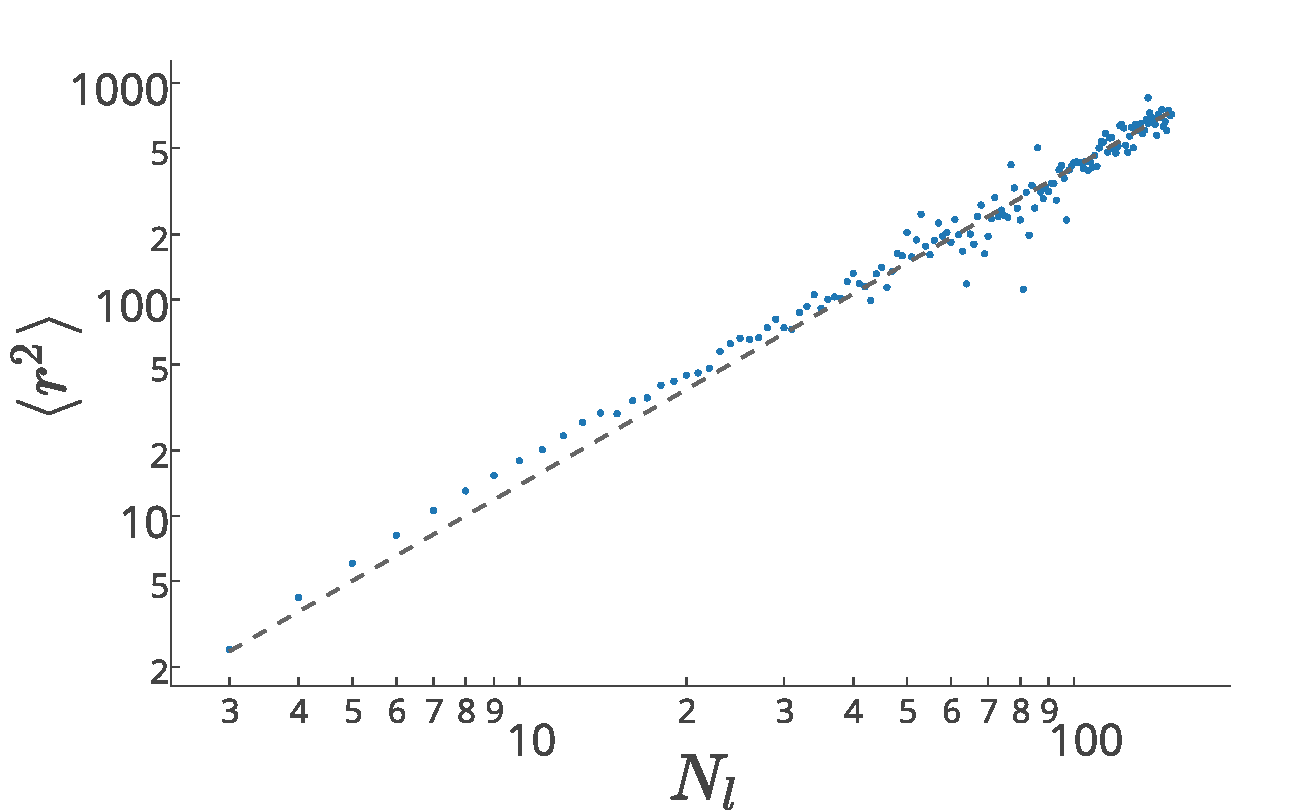
\includegraphics[width=\linewidth]{r_squared.pdf}
\captionof{figure}{Average end to end distance $\langle r^2\rangle$ as a function of polymer beads $N$ on a log scale. The blue dots depict $\langle r^2\rangle$ and the dashed line is fitted to $\langle r^2\rangle$ with $a\cdot N^{2\nu}$. The fitted value for $2\nu = 1.469 \pm 0.04246$.}
\label{fig:r_squared}
\end{Figure}

\subsection{Some notes on the program}
The energy calculations, LJ potential and bending energy, are for better performance written in Fortran. To make a connection between the Fortran code and the Python program, an interface is made using \emph{Fortran to Python interface generator} (F2PY). F2PY creates a Python C/API extension module that makes it possible to call the in Fortran written energy subroutine.